\scanpage{4}
\mspage{\unsure{63|68}}
\deleted{
a) La fonction $\rho_r$ sur S est semi-continue inférieurement, la
fonction $\rho_n$ sur S est semi-continue supérieurement, donc la fonction
$\rho_u=\rho_n-\rho_r$ est semi-continue supérieurement.

b) Les \deleted{\unsure{c}}conditions suivantes (stables par changement de base
quelconque) sont équivalentes:

(i) La fonction $\rho_r$ sur S est localement constante.

(ii) Il existe localement, au sens de la topologie étale,
un tore maximal dans G.

(ii bis) Il existe localement, au sens de la topologie
fidèlement plate quasi-compacte, un tore maximal dans G.

c) Soient $T_1,T_2$ deux tores maximaux dans G (ce qui implique que
l'on est sous les conditions envisagées dans b). Alors $T_1,T_2$ sont
\figure{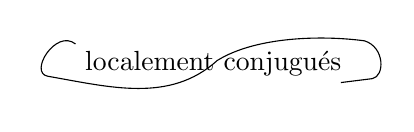
\begin{tikzpicture}[baseline=(t.base)]
\node[inner sep=2pt] (t) {localement conjugués};
\draw (-1.75,.25) .. controls (-2,.45) and (-2.35,-.12) .. (-2.1,-.16)
.. controls (-1.3,-.3) and (-.55,-.5) .. (.05,.04)
.. controls (.55,.35) and (1.4,.36) .. (1.92,.29)
.. controls (2.18,.21) and (2.18,-.16) .. (2.02,-.19)
--(1.62,-.24);
\end{tikzpicture}}
au sens de la topologie étale, i.e. il existe
un morphisme étale surjectif $S'\to S$ tel que les sous-groupes $T_{1\,S'}$ et
$T_{2\,S'}$ de $G_{S'}$ soient conjugués par une section de $G_{S'}$ sur $S'$.

d) Sous les conditions de b), i.e. lorsque $\rho_r$ est localement
constante, il en est de même de $\rho_n$ (donc aussi de $\rho_u=\rho_n-\rho_r$).

Démonstration.

a) Notons que pour tout morphisme $S'\to S$, si $G'=G\times_S S'$, les
fonctions $\rho'_r$ etc sur $S'$ \deleted{construites à l'aide} définies en termes de
G' comme $\rho_r$ etc en termes de G, s'obtiennent simplement \deleted{comme} en composant
ces dernières avec $S'\to S$. Lorsque $S'\to S$ est fidèlement plat quasi
compact, il en résulte que $\rho'$ est continue, resp. semi-continue
supérieurement, resp. semi-continue inférieurement, si et seulement si
$\rho$ l'est, \deleted{(SGA VIII} la topologie \inserted{de Zariski} de S étant en effet quotient de celle
de S' (SGA VIII 4.3.). Par suite, les assertions de a) sont locales pour
}
\margin{3}
